\chapter{Arhitektura i dizajn sustava}
		
		\textbf{\textit{dio 1. revizije}}\\

		
		Arhitekturu sustava možemo podijeliti na tri podsustava:
		\begin{itemize}
			\item Web preglednik
			\item Web poslužitelj
			\item Baza podataka
		\end{itemize}
	
		
		%unos slike
		\begin{figure}[H]
			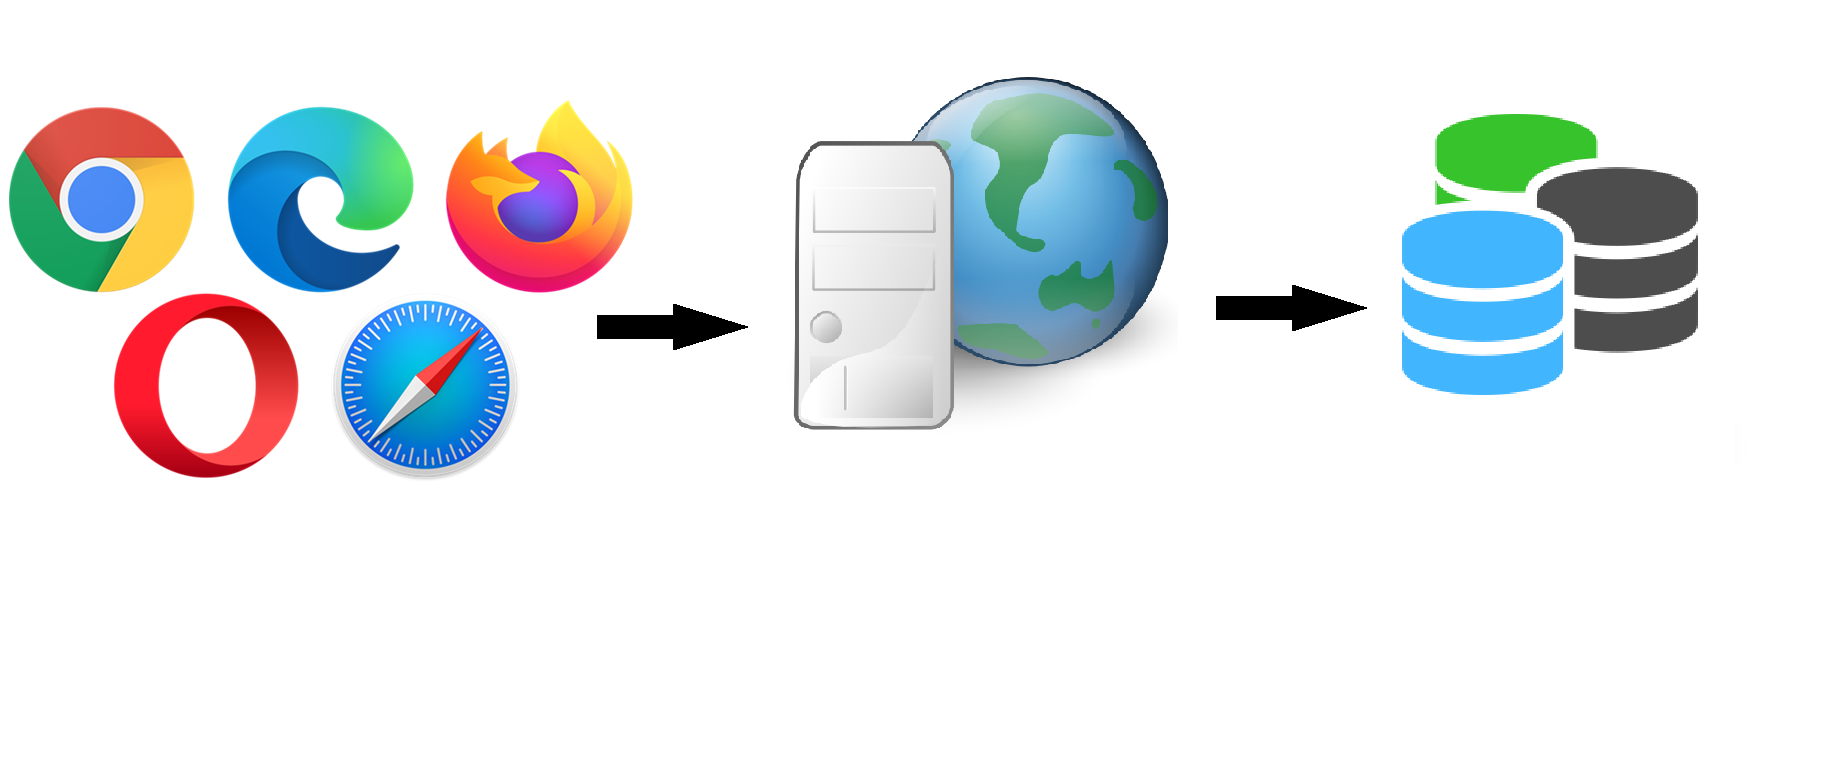
\includegraphics[scale=0.35]{slike/arhitektura.png} %veličina slike u odnosu na originalnu datoteku i pozicija slike
			\centering
			\caption {Arhitektura sustava}
			\label{fig:promjene}
		\end{figure}
		
		Korisnik pomoću web preglednika po vlastitom izboru dobiva mogućnost  pristupa web aplikaciji na  Internetu. Preglednik zapravo šalje zahtjev HTTP protokolom web poslužitelju na kojem se nalazi web aplikacija i on ju pokreće i omogućuje korisniku daljnji rad na aplikaciji.
		
		Pred korisnikom se nalaze sve funkcionalnosti koje aplikacija pruža. On svojevoljno odabire pojedinu fukcionalnost te tako šalje zahtjev aplikaciji koja pristupa bazi podataka i prikuplja zatražene podatke i osvježava mu pregled aplikacije s prikupljenim podacima. 

		Sama aplikacija je sastavljena po načelu objektno usmjerene arhitekture. Razlog odabira takve arhitekture je trenutna sveprisutnost u industriji te predstavlja standard razvoja složenih programskih zahtjeva. Budući da je razvoj aplikacije zamišljen kao rad više ljudi u timu  objektno usmjerena arhitektura nudi da se sustav logički razdijeli na više cjelina te time omogućuje paralelnost razvoja.
		Također nudi recikliranje koda, mogućnost dodavanja novih funkcionalnosti bez poteškoća i greške se lako detektiraju i ispravljaju.
		
		Aplikacija je razvijena u programskom jeziku Java 11 te kao razvojni okvir koristi Java Spring Boot verzije 2.3.4. Za sigurnost i sprječavanje vanjskih napada koristi se Spring Security.
		Kako bi se olakšala komunikacija s bazom koristi se Spring JPA.  
		Za razvojno okruženje koristi se Ecplise, IntelliJ i VSCode.
		 
		
		Frontend je pisan u  React-u. React je open-source, frontend, JavaScript knjižnica koja služi  za izgradnju korisničkog sučelja. Koristi HTML, CSS, JSX i JavaScript kako bi modelirao sučelje.
		
		Komunikacija između Jave na backendu i Reacta na frontendu je omogućena korištenjem REST api-ja.
			%unos slike
		\begin{figure}[H]
			
\includegraphics[scale=0.7]{slike/arhitektura2.jpg} %veličina slike u odnosu na originalnu datoteku i pozicija slike
			\centering
			\caption {Arhitektura sustava}
			\label{fig:promjene}
		\end{figure}
	
			\begin{figure}[H]
			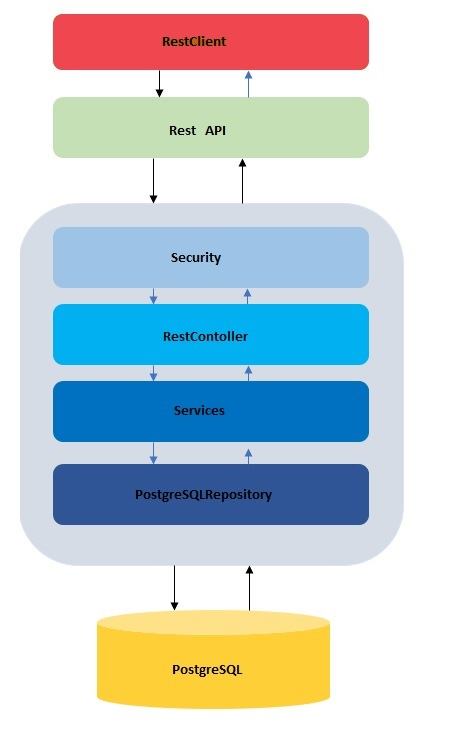
\includegraphics[scale=0.9]{slike/arhitektura3.jpg} %veličina slike u odnosu na originalnu datoteku i pozicija slike
			\centering
			\caption {Arhitektura sustava}
			\label{fig:promjene}
		\end{figure}

		\newpage	
		\section{Baza podataka}
			
			\textbf{\textit{dio 1. revizije}}\\
		
		Implementacija baze podataka ostvarena je uporabom PostgreSQL zbog jednostavnosti korištenja i pozitivnog iskustva članova tima. 
		
		Baza podataka sastoji se od sljedećih tablica:
		
		\begin{packed_item}
			\item Korisnik
			\item Zahtjev
			\item Lokacija
			\item Kandidatura
			\item Kandidiranje
			\item Ocjenjivanje
			\item ImaUlogu 
			\item Uloga
			
		\end{packed_item}
		
			\subsection{Opis tablica}
			
					    \textbf{ Korisnik}
		    \text Ovaj entitet sadržava sve važne informacije o korisniku aplikacije. Sadrži atribute: ID${\_}$Korisnik, ime, prezime, email, lozinka, aktivan, token, slika te ID${\_}$Lokacija. Ovaj entitet je u vezi \emph{One-to-Many} s entitetom Zahtjev preko atributa ID${\_}$Korisnik gdje korisnik ima dvije uloge, u vezi  \emph{Many-to-One} s entitetom Lokacija preko atributa ID${\_}$Lokacija, u vezi \emph{Many-to-Many} s entitetom Kandidatura preko vezne tablice Kandidiranje i atributa ID${\_}$Korisnik, u vezi \emph{One-to-Many} s entitetom Ocjenjivanje preko atributa ID${\_}$Korisnik gdje korisnik ima dvije uloge te u vezi \emph{Many-to-Many} s entitetom Uloga preko vezne tablice ImaUlogu i atributa ID${\_}$Korisnik
				
				\begin{longtabu} to \textwidth {|X[6, l]|X[6, l]|X[20, l]|}
					
					\hline \multicolumn{3}{|c|}{\textbf{Korisnik}}	 \\[3pt] \hline
					\endfirsthead
					
					\hline \multicolumn{3}{|c|}{\textbf{Korisnik }}	 \\[3pt] \hline
					\endhead
					
					\hline 
					\endlastfoot
					
					\colorbox{LightGreen}{\textbf{ID${\_}$Korisnik}} & BIGSERIAL & jedinstveni identifikator korisnika 	 	\\ \hline
					ime & VARCHAR	&  ime korisnika	\\ \hline 
					prezime & VARCHAR	& prezime korisnika 		\\ \hline
					email & VARCHAR & e-mail adresa korisnika  \\ \hline 
					lozinka	& VARCHAR & hash lozinke 	\\ \hline  
					aktivan & BOOLEAN & status korisnika \\ \hline
					token & VARCHAR & JWT refresh token koji se koristi pri autentifikaciji korisnika \\ \hline
					slika & VARCHAR & putanja do fotografije korisnika \\ \hline
					\colorbox{LightBlue}{\underline{ID${\_}$Lokacija} }& BIGINT & identifikator lokacije \\ \hline
					
				\end{longtabu}
				    \textbf{Zahtjev}
			    \text Ovaj entitet sadržava sve važne informacije o korisnikovu zahtjevu. Sadrži atribute: ID${\_}$Zahtjev, opis, tstmp, status, brojMobitela, ID${\_}$Autor, ID${\_}$Izvrsitelj, primljenaNotif, ID${\_}$Lokacija, execTstmp. Ovaj entitet je u vezi \emph{Many-to-one} s entitetom Lokacija preko atributa ID${\_}$Lokacija, također u vezi \emph{One-to-Many} s entitetom Ocjenjivanje preko atributa ID${\_}$Zahtjev te u dvije veze \emph{Many-to-One} s entitetom Korisnik preko atributa ID${\_}$Korisnik što rezultira pojavom atributa ID${\_}$Autor i ID${\_}$Izvrsitelj u tablici Zahtjev.  
			
				\begin{longtabu} to \textwidth {|X[6, l]|X[6, l]|X[20, l]|}
					
					\hline \multicolumn{3}{|c|}{\textbf{Zahtjev}}	 \\[3pt] \hline
					\endfirsthead
					
					\hline \multicolumn{3}{|c|}{\textbf{Zahtjev }}	 \\[3pt] \hline
					\endhead
					
					\hline 
					\endlastfoot
					
					\colorbox{LightGreen}{\textbf{ID${\_}$Zahtjev}} & BIGSERIAL	&  jedinstveni identifikator zahtjeva	 	\\ \hline
					opis & VARCHAR	& opis zahtjeva 		\\ \hline 
					tstmp & TIMESTAMP	& vremenska točka do kada se treba izvršiti zahtjev	\\ \hline
					status	& VARCHAR & status zahtjeva  	\\ \hline
					brojMobitela & VARCHAR & broj mobitela autora zahtjeva \\ \hline
					\colorbox{LightBlue}{\underline{ID${\_}$Autora}} & BIGINT & jedinstveni identifikator korisnika(autora zahtjeva) \\ \hline
					\colorbox{LightBlue}{\underline{ID${\_}$Izvrsitelj}} & BIGINT & jedinstveni identifikator korisnika(izvršitelja zahtjeva) \\ \hline
					primljenaNotif & BOOLEAN & zastavica status notifikacije \\ \hline
					\colorbox{LightBlue}{\underline{ID${\_}$Lokacija}} & BIGINT & identifikator lokacije \\ \hline
					execTstmp & TIMESTAMP & točka u vremenu kada je zahtjev izvršen \\ \hline
					
				
				\end{longtabu}
			
			    \newpage
						    \textbf{Lokacija}
			    \text Ovaj entitet sadržava sve važne informacije o lokaciji. Sadrži atribute: ID${\_}$Lokacija, duljina i sirina, drzava, naselje te adresa. Ovaj entitet je u vezi \emph{One-to-Many} s entitetom Zahtjev preko atributa ID${\_}$Lokacija, također je u vezi \emph{One-to-Many} s entitetom Korisnikom preko atributa ID${\_}$Lokacija te u vezi \emph{One-to-Many} s entitetom Kandidatura preko atributa ID${\_}$Lokacija. 
			
				\begin{longtabu} to \textwidth {|X[6, l]|X[6, l]|X[20, l]|}
					
					\hline \multicolumn{3}{|c|}{\textbf{Lokacija}}	 \\[3pt] \hline
					\endfirsthead
					
					\hline \multicolumn{3}{|c|}{\textbf{Lokacija }}	 \\[3pt] \hline
					\endhead
					
					\hline 
					\endlastfoot
					\colorbox{LightGreen}{\textbf{ID${\_}$Lokacija}} & BIGSERIAL & jedinstveni identifikator lokacije \\ \hline
					duljina & NUMERIC	& geografska dužina \\ \hline
					sirina & NUMERIC & geografska sirina \\ \hline
					drzava & VARCHAR	& naziv države 		\\ \hline
					naselje & VARCHAR & naziv naselja  \\ \hline 
					adresa	& VARCHAR & adresa na kojoj treba odraditi zahtjev	\\ \hline 	
					
				\end{longtabu}
			
			\textbf{ Kandidatura}
		    \text Ovaj entitet sadržava sve važne informacije o kandidaturi za korisnika godine. Sadrži atribute: ID${\_}$Kandidatura, godina i ID${\_}$Lokacija. Ovaj entitet je u vezi \emph{Many-to-Many} s entitetom Korisnik preko vezne tablice Kandidiranje i atributa ID${\_}$Kandidatura te u vezi \emph{Many-to-One} s Lokacijom preko atributa ID${\_}$Lokacija.

				\begin{longtabu} to \textwidth {|X[7, l]|X[6, l]|X[20, l]|}
					
					\hline \multicolumn{3}{|c|}{\textbf{Kandidatura}}	 \\[3pt] \hline
					\endfirsthead
					
					\hline \multicolumn{3}{|c|}{\textbf{Kandidatura}}	 \\[3pt] \hline
					\endhead
					
					\hline 
					\endlastfoot
					
					\colorbox{LightBlue}{\underline{ID${\_}$Lokacija}} & BIGINT & identifikator lokacije  \\ \hline
					godina & INT & godina kandidature  \\[3pt] \hline 
					\colorbox{LightGreen}{\textbf{ID${\_}$Kandidatura}} & BIGSERIAL	& jedinstveni identifikator lokacije  \\ \hline
				
					
				\end{longtabu}
				
				\textbf{Kandidiranje}
		    \text Ovaj entitet je vezna tablica koja povezuje entitete Korisnik i Kandidatura. Sadrži dva strana ključa: ID${\_}$Korisnik i ID${\_}$Kandidatura.
		    
		    	\begin{longtabu} to \textwidth {|X[7, l]|X[6, l]|X[20, l]|}
		    		
		    		\hline \multicolumn{3}{|c|}{\textbf{Kandidiranje}}	 \\[3pt] \hline
		    		\endfirsthead
		    		
		    		\hline \multicolumn{3}{|c|}{\textbf{Kandidiranje}}	 \\[3pt] \hline
		    		\endhead
		    		
		    		\hline 
		    		\endlastfoot
		    		\colorbox{LightGreen}{\textbf{\underline{ID${\_}$Korisnik}}} & BIGINT	& identifikator korisnika 	 	\\ \hline
		    		\colorbox{LightGreen}{\textbf{\underline{ID${\_}$Kandidatura}}} & BIGINT	& identifikator kandidature  \\ \hline
		    		
		    	\end{longtabu}
		    
		    \newpage
		    
		        \textbf{Ocjenjivanje}
		    \text Ovaj entitet sadržava sve važne informacije o međusobnom ocjenjivanju korisnika. Sadrži atribute: ID${\_}$Ocjenjivanje, ID${\_}$Zahtjev, ocjena, komentar, ID${\_}$Ocjenjivac i ID${\_}$Ocjenjeni. Ovaj entitet je u dvostrukoj vezi \emph{Many-to-One} s entitetom Korisnik preko atributa ID${\_}$Ocjenjeni i ID${\_}$Ocjenjivac te u vezi \emph{Many-to-One} s entitetom Zahtjev preko atributa ID${\_}$Zahtjev.
		    
				\begin{longtabu} to \textwidth {|X[7, l]|X[6, l]|X[20, l]|}
					
					\hline \multicolumn{3}{|c|}{\textbf{Ocjenjivanje}}	 \\[3pt] \hline
					\endfirsthead
					
					\hline \multicolumn{3}{|c|}{\textbf{Ocjenjivanje }}	 \\[3pt] \hline
					\endhead
					
					\hline 
					\endlastfoot
					
					\colorbox{LightGreen}{\textbf{ID${\_}$Ocjenjivanje}} & BIGSERIAL & jedinstveni identifikator ocjenjivanja 	\\ \hline	
					\colorbox{LightBlue}{\underline{ID${\_}$Zahtjev}} & BIGINT	&  identifikator zahtjeva	 	\\ \hline
					ocjena & INT	&  ocjena usluge		\\ \hline 
					komentar & VARCHAR	& komentar ocjenitelja 		\\ \hline
					\colorbox{LightBlue}{\underline{ID${\_}$Ocjenjivac}} & BIGINT	& identifikator ocjenjivaca 	\\ \hline
					\colorbox{LightBlue}{\underline{ID${\_}$Ocjenjeni}} & BIGINT	& identifikator ocjenjenog 	\\ \hline
					
				\end{longtabu}
			
			
		
			\textbf{Uloga}
			\text Entitet sadržava informaciju o ulozi korisnika tijekom korištenja aplikacije. Uloga može biti administrator ili obični korisnik. Sadrži atribute: ID${\_}$Uloga i naziv. U vezi je \emph{Many-to-Many} s entitetom Korisnik preko vezne tablice ImaUlogu i atributa ID${\_}$Uloga.
			
			\begin{longtabu} to \textwidth {|X[6, l]|X[6, l]|X[20, l]|}
				
				\hline \multicolumn{3}{|c|}{\textbf{Uloga}}	 \\[3pt] \hline
				\endfirsthead
				
				\hline \multicolumn{3}{|c|}{\textbf{Uloga }}	 \\[3pt] \hline
				\endhead
				
				\hline 
				\endlastfoot
				
				\colorbox{LightGreen}{\textbf{ID${\_}$Uloga}}& BIGSERIAL &  jedinstveni identifikator uloge	 	\\ \hline
				naziv & VARCHAR	& naziv uloge 	\\ \hline
				
				
			\end{longtabu}
		
			\textbf{ImaUlogu}
			\text je vezna tablica koja sadržava informacije koji korisnik ima koju ulogu unutar aplikacije. Sadrži atribute - strane ključeve: ID${\_}$Korisnik i ID${\_}$Uloga.
			
			\begin{longtabu} to \textwidth {|X[6, l]|X[6, l]|X[20, l]|}
				
				\hline \multicolumn{3}{|c|}{\textbf{ImaUlogu}}	 \\[3pt] \hline
				\endfirsthead
				
				\hline \multicolumn{3}{|c|}{\textbf{ImaUlogu }}	 \\[3pt] \hline
				\endhead
				
				\hline 
				\endlastfoot
				\colorbox{LightGreen}{\textbf{\underline{ID${\_}$Korisnik}}} & BIGINT	& identifikator korisnika 	 	\\ \hline
				\colorbox{LightGreen}{\textbf{\underline{ID${\_}$Uloga}}} & BIGINT	&  identifikator uloge	 	\\ \hline
				
				
				
			\end{longtabu}
		
		   \newpage
			\subsection{Dijagram baze podataka}
			
			
			%unos slike
			\begin{figure}[H]
				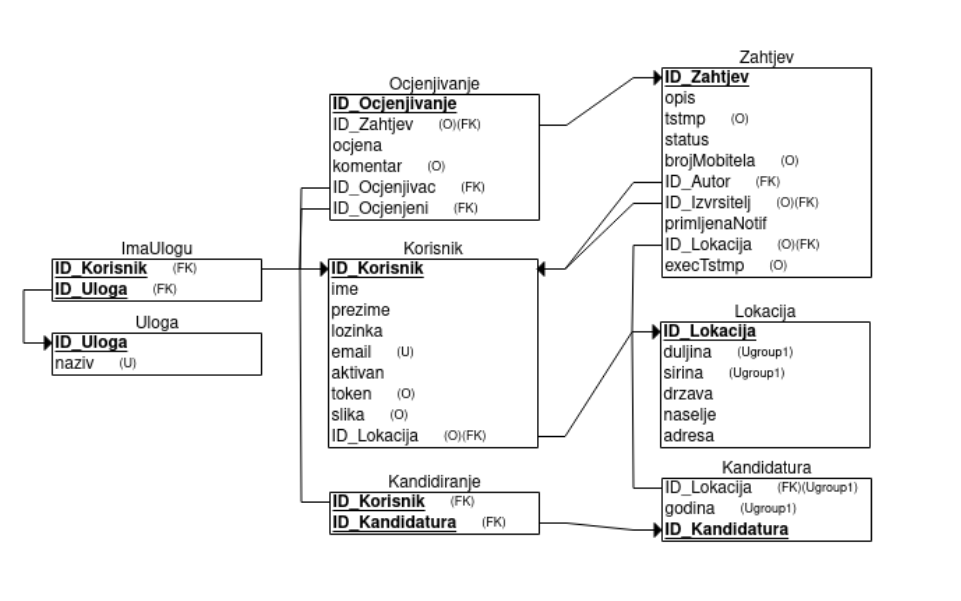
\includegraphics[scale=0.5]{slike/REL_DIJAGRAM.png} %veličina slike u odnosu na originalnu datoteku i pozicija slike
				\centering
				\caption {Dijagram baze podataka}
				\label{fig:promjene}
			\end{figure}
			
			\eject
			
		\section{Dijagram razreda}
		
			\textit Na slikama  \ref{fig:4.5}, \ref{fig:4.6}, \ref{fig:4.7}, \ref{fig:4.8} i \ref{fig:4.9} su prikazani dijagrami razreda za backend. Raspoređeni su u više slika radi bolje preglednosti i slične funkcionalnosti. Iz samih slika lakše se može uočiti povezanost samih stavki, njihova ovisnost te sadržaj atributa i funkcionalnosti.
			%unos slike
			\begin{figure}[H]
				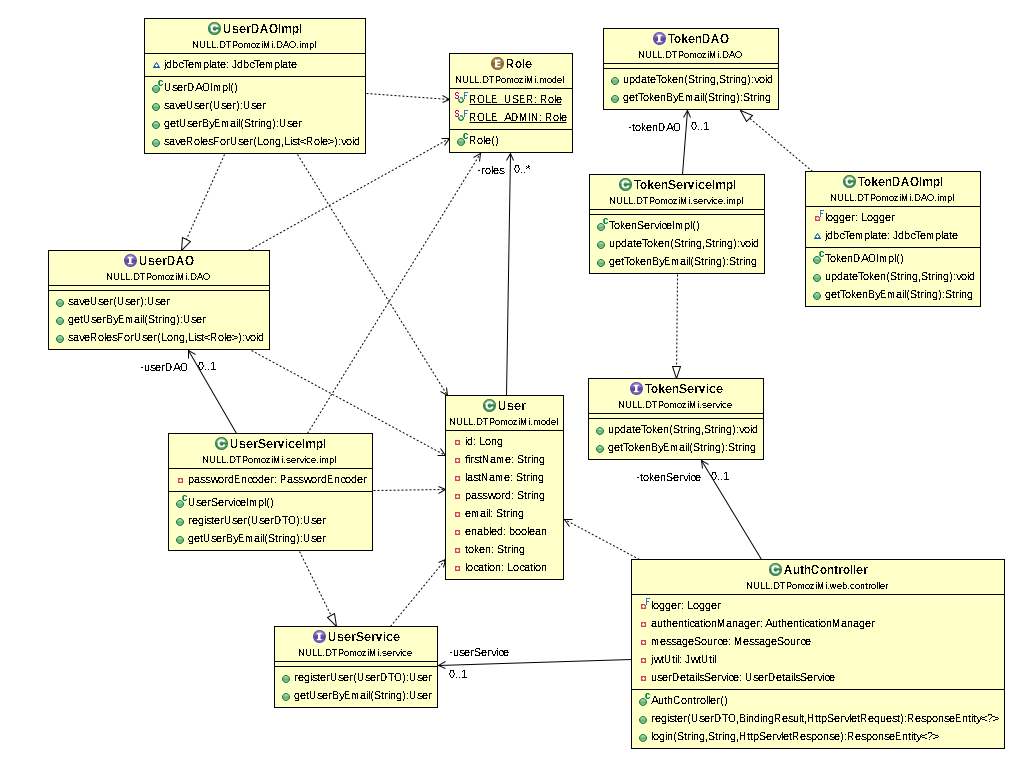
\includegraphics[scale=0.65]{slike/user.png} %veličina slike u odnosu na originalnu datoteku i pozicija slike
				\centering
				\caption { Dijagram razreda za User}
				\label{fig:4.5}
			\end{figure}
		
			%unos slike
			\begin{figure}[H]
				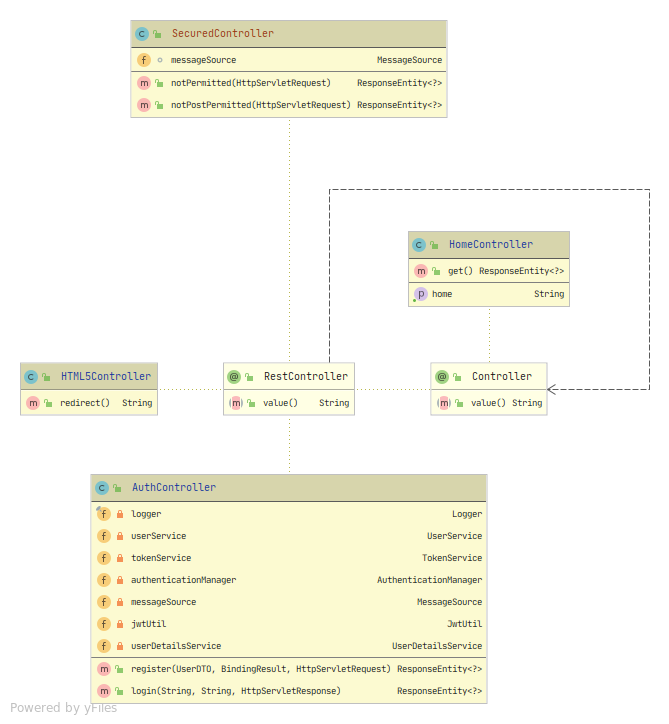
\includegraphics[scale=0.65]{slike/ControllersDiagram.png} %veličina slike u odnosu na originalnu datoteku i pozicija slike
				\centering
				\caption { Dijagram razreda za controllere}
				\label{fig:4.6}
			\end{figure}
			
			%unos slike
			\begin{figure}[H]
				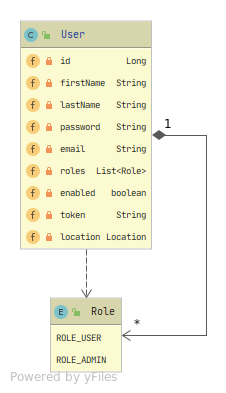
\includegraphics[scale=0.65]{slike/ModelUml.png} %veličina slike u odnosu na originalnu datoteku i pozicija slike
				\centering
				\caption { Dijagram razreda za model korisnika}
				\label{fig:4.7}
			\end{figure}
			
			
			%unos slike
			\begin{figure}[H]
				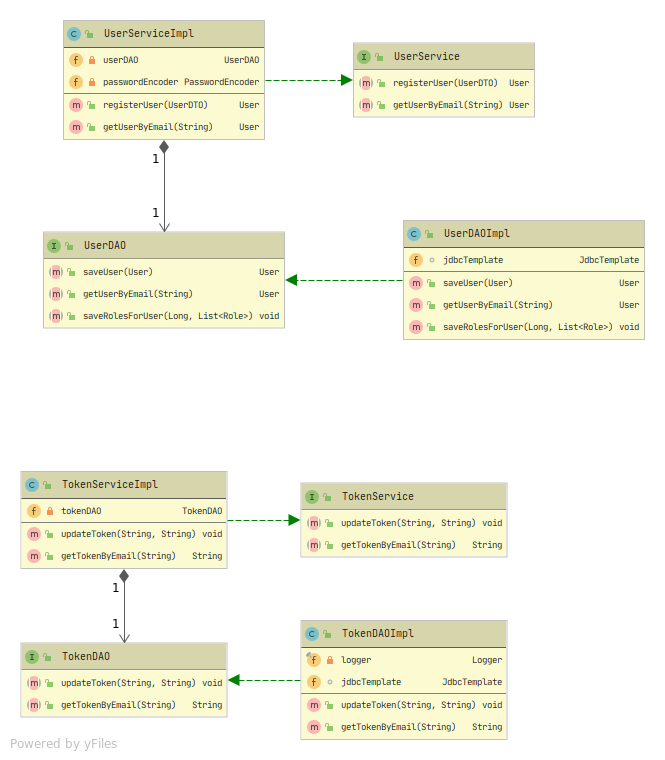
\includegraphics[scale=0.65]{slike/ServiceDaoUml.png} %veličina slike u odnosu na originalnu datoteku i pozicija slike
				\centering
				\caption { Dijagram razreda za ServiceDao}
				\label{fig:4.8}
			\end{figure}
			
			
			%unos slike
			\begin{figure}[H]
				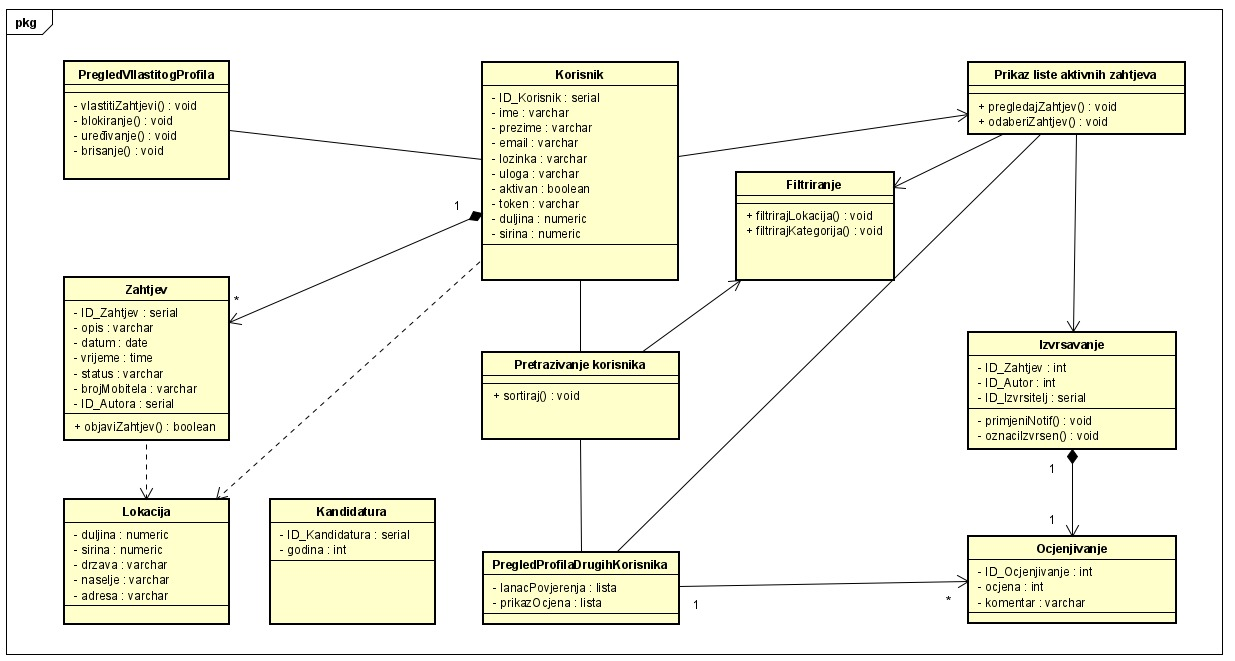
\includegraphics[scale=0.4]{slike/class_dijagram.jpeg} %veličina slike u odnosu na originalnu datoteku i pozicija slike
				\centering
				\caption { Dijagram razreda - models}
				\label{fig:4.9}
			\end{figure}
			
			
			\begin{comment}
			\textbf{\textit{dio 2. revizije}}\\			
			
			\textit{Prilikom druge predaje projekta dijagram razreda i opisi moraju odgovarati stvarnom stanju implementacije}
			\end{comment}
\newpage			
\section{Dijagram stanja}
			
			\textbf{\textit{dio 2. revizije}}\\		
		
		\text Dijagram stanja prikazuje stanja objekta te prijelaze iz jednog stanja u drugo temeljene na dogadajima. Na slici
		\ref{fig:4.10} prikazan je dijagram stanja registriranog korisnika. Nakon prijave, korisniku se prikazuje početna stranica(Home page). Korisnik klikom na Profil otvara svoju profilnu stranicu. Korisnik može odabirom Aktivni Zahtjevi pregledati vlastite zahtjeve aktivne zahtjeve. Isto tako odabirom Izvršeni Zahtjevi može pregledati vlastite zahtjeve koji su Izvršeni. Korisniku se klikom na Pregled Zahtjeva nudi pregled aktivnih zahtjeva te mogućnost odabira nekoga od zahtjeva s liste. Nakon izvršavanja zahtjeva korisnik mora ocijeniti drugog korisnika i opcionalno ostaviti komentar te se komentari i ocjene vide u profilu korisnika. Korisniku se nudi i mogućnost uređivanja osobnih podataka kao i brisanje korisničkog računa, dok klikom  na Search korisnik može pretraživati druge korisnike aplikacije. Također klikom na Zadavanje Zahtjeva korisnik može zadati novi zahtjev.
		
			%unos slike
		\begin{figure}[H]
			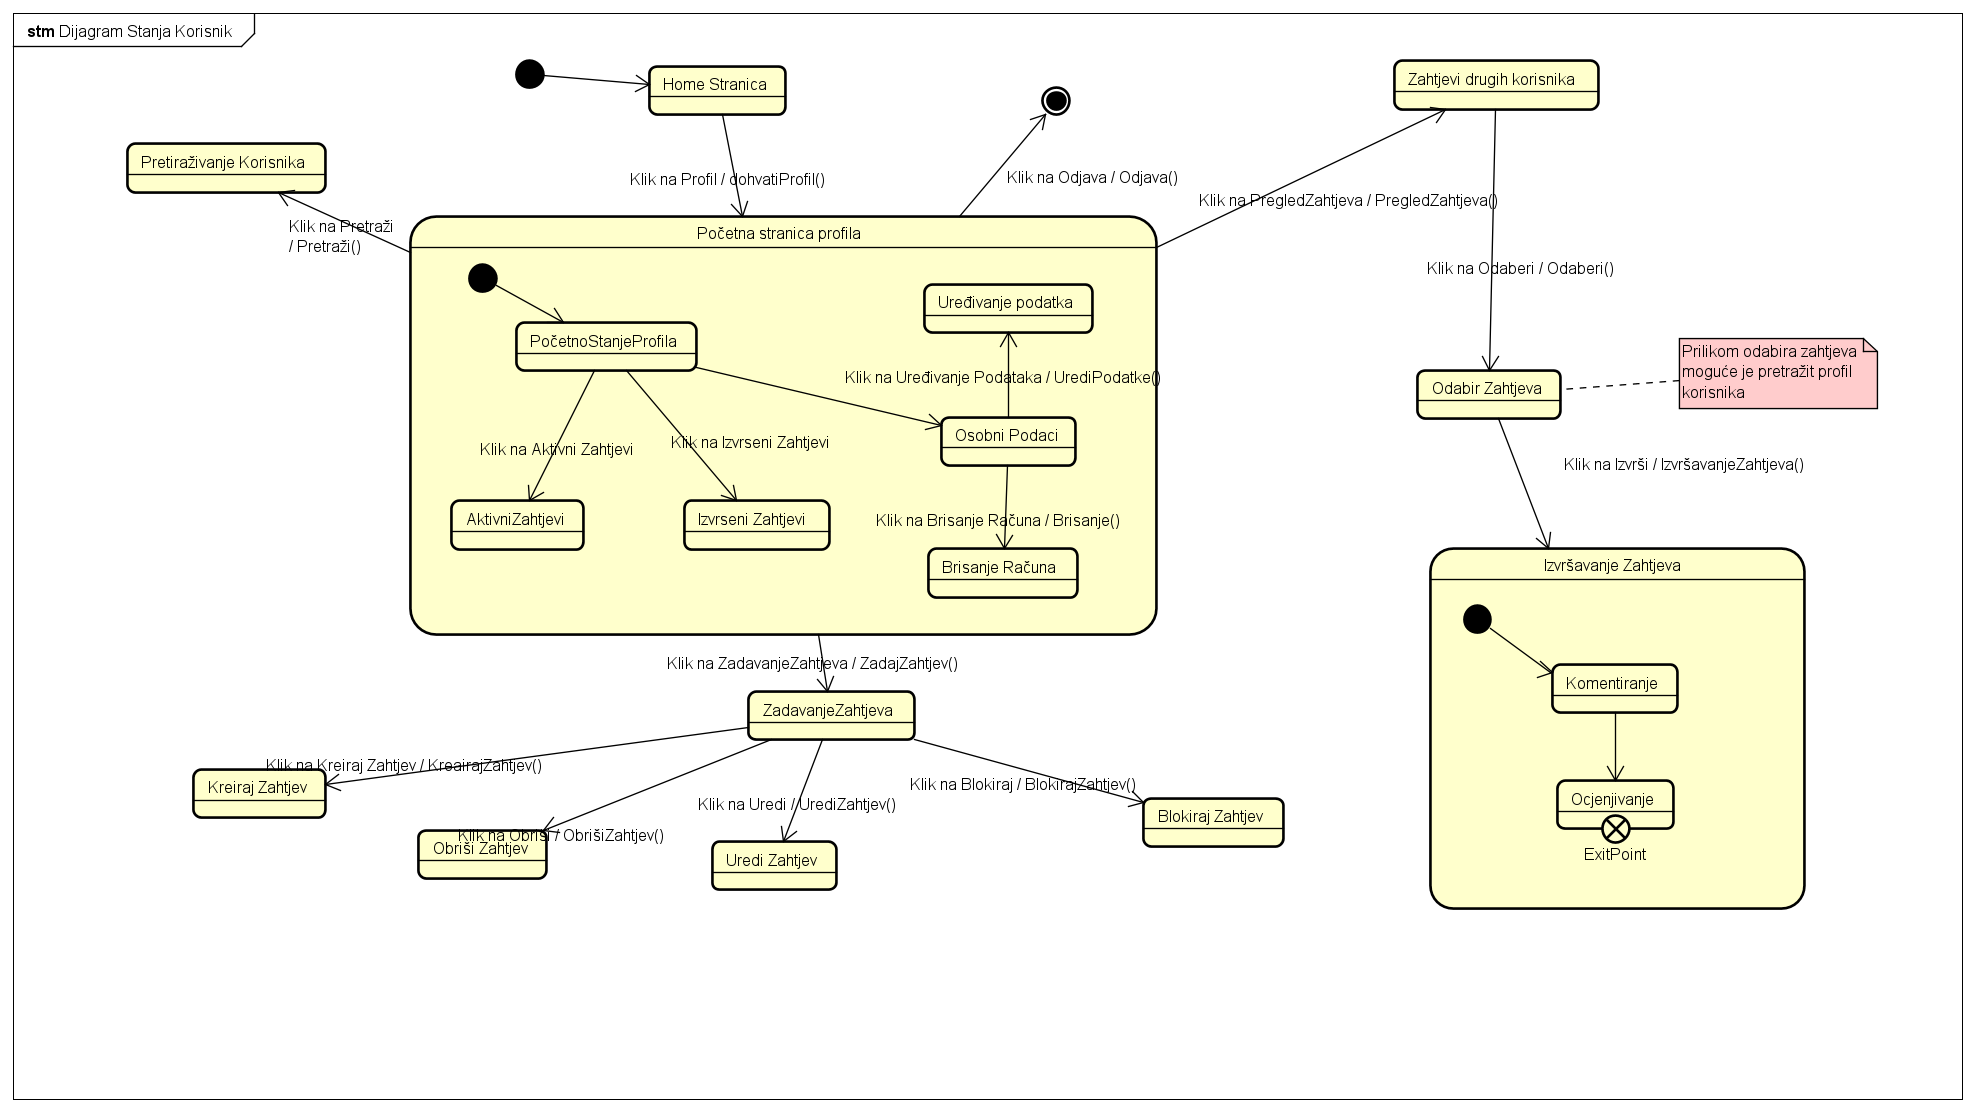
\includegraphics[scale=0.3]{slike/Dijagram Stanja.png} %veličina slike u odnosu na originalnu datoteku i pozicija slike
			\centering
			\caption { Dijagram stanja}
			\label{fig:4.10}
			\end{figure}		
			
\begin{comment}		
		\section{Dijagram stanja}
			
			
			\textbf{\textit{dio 2. revizije}}\\
			
			\textit{Potrebno je priložiti dijagram stanja i opisati ga. Dovoljan je jedan dijagram stanja koji prikazuje \textbf{značajan dio funkcionalnosti} sustava. Na primjer, stanja korisničkog sučelja i tijek korištenja neke ključne funkcionalnosti jesu značajan dio sustava, a registracija i prijava nisu. }
			
			
			\eject 
\end{comment}
\newpage
		\section{Dijagram aktivnosti}
			
			\textbf{\textit{dio 2. revizije}}\\
			
			\text Dijagram aktivnosti primjenjuje se za opis modela toka upravljanja ili toka podataka. Ne upotrebljava se za modeliranje dogadajima poticanog ponašanja. U modeliranju toka upravljanja svaki novi korak poduzima se nakon završenog prethodnog, a naglasak je na jednostavnosti. Na dijagramu \ref{fig:4.11} prikazan je proces izvršavanja zahtjeva za pomoć. Korisnik se prijavljuje u sustav,prikazujemu se početna stranica, nakon koje on odabire Pregled zahtjeva. Kada je zamijetio zahtjev kojeg može izvršiti, odabire taj zahtjev te mu se poslužuju dodatne informacije o zahtjevu kako bi mogao izvršiti zahtjev. Nakon izvršenog zahtjeva, korisnik treba ocijeniti i opcinalno komentirati.
			
			
						%unos slike
		\begin{figure}[H]
			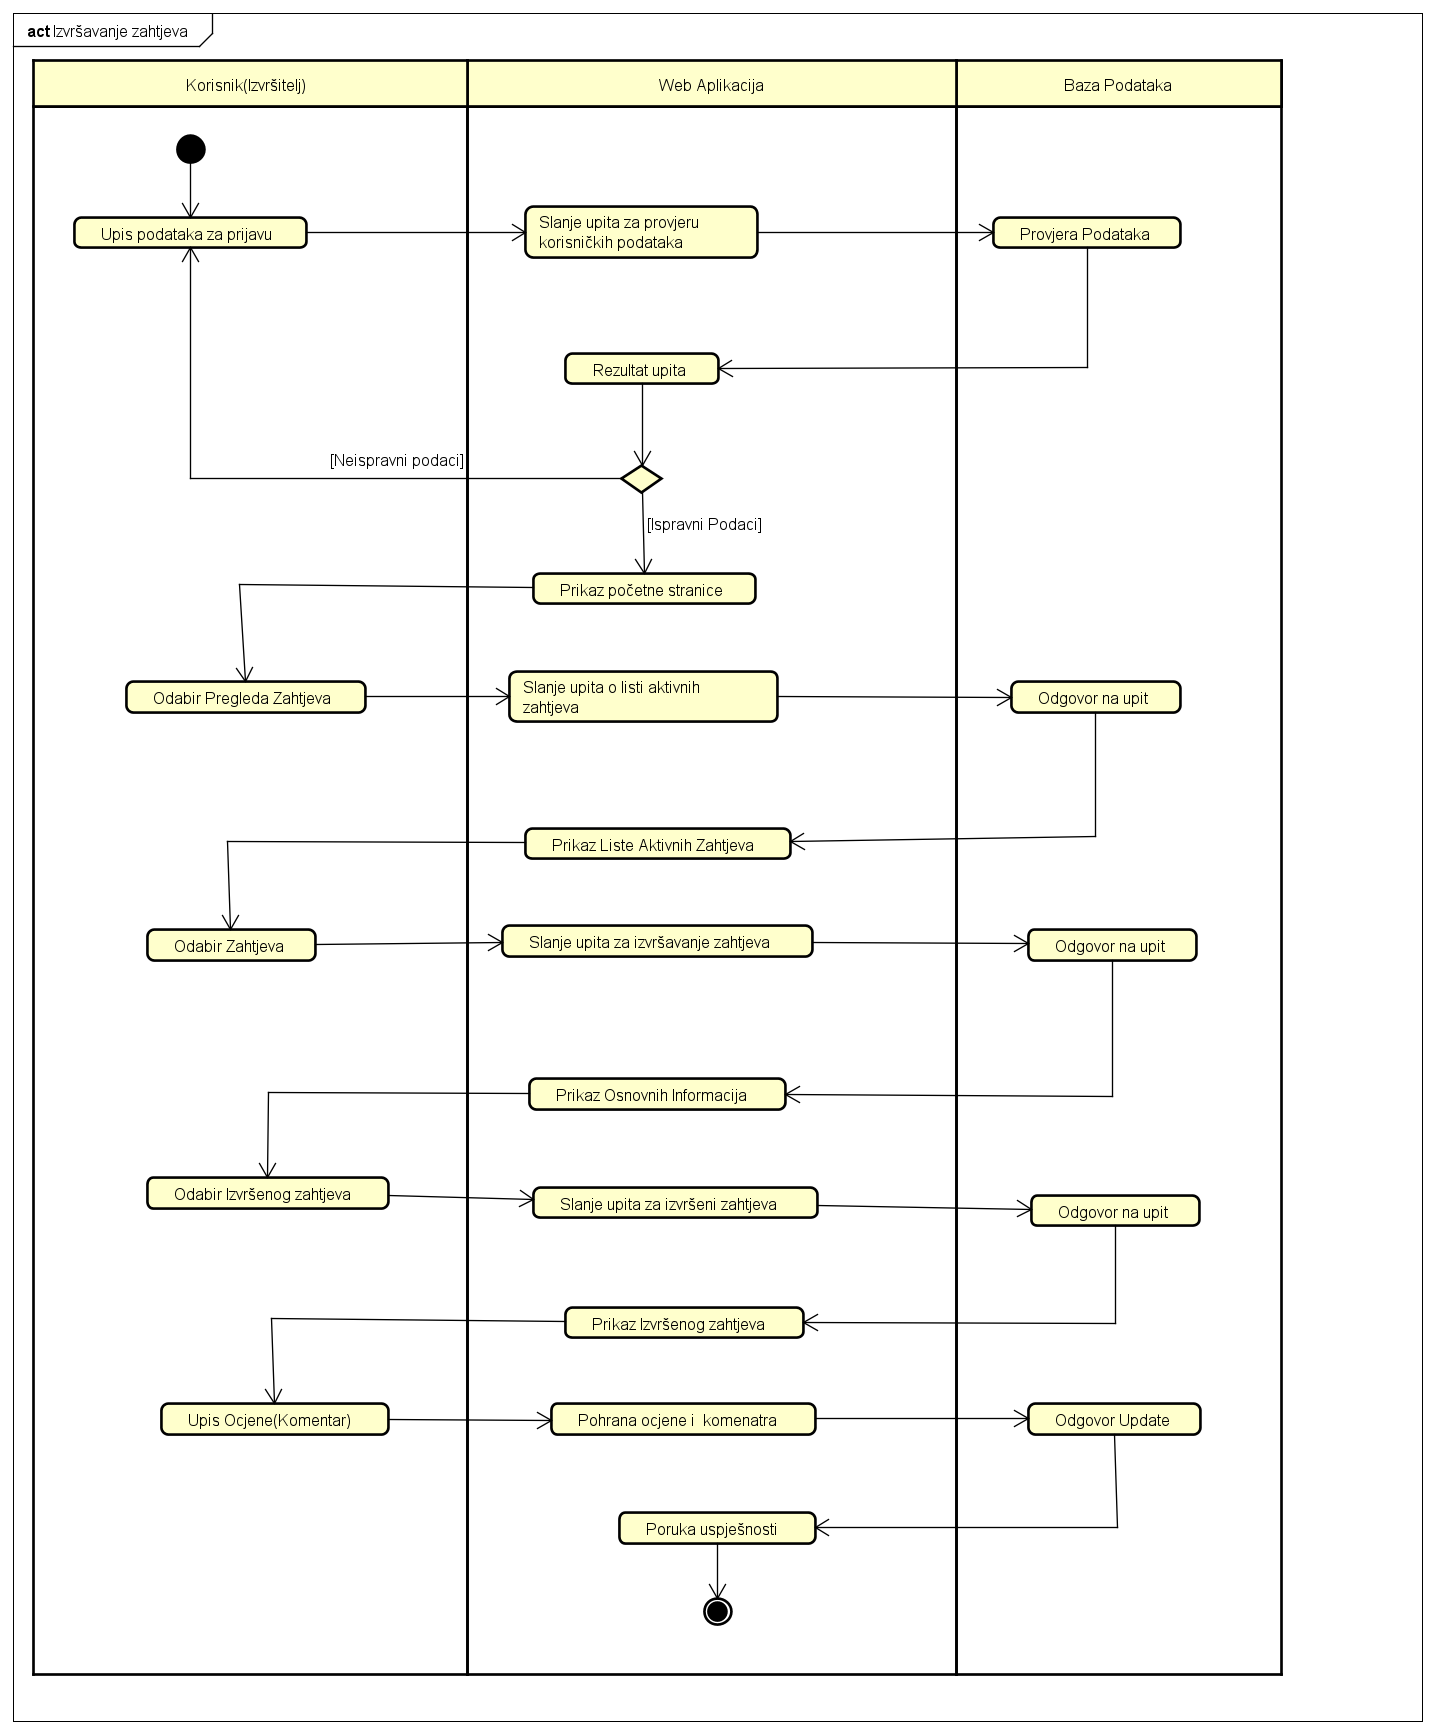
\includegraphics[scale=0.3]{slike/DijagramAktivnosti.png} %veličina slike u odnosu na originalnu datoteku i pozicija slike
			\centering
			\caption { Dijagram Aktivnosti}
			\label{fig:4.11}
			\end{figure}

\begin{comment}
		\section{Dijagram aktivnosti}
			
			\textbf{\textit{dio 2. revizije}}\\
			
			 \textit{Potrebno je priložiti dijagram aktivnosti s pripadajućim opisom. Dijagram aktivnosti treba prikazivati značajan dio sustava.}
			
			\eject
\end{comment}
\newpage
		\section{Dijagram komponenti}
		
			\textbf{\textit{dio 2. revizije}}\\
			
			\text   Dijagram komponenti prikazan na slici \ref{fig:4.12} opisuje organizaciju i meduovisnost
            komponenti, interne strukture i odnose prema okolini. Sustavu se pristupa preko dva različita sučelja. Preko sučelja za dohvat HTML, CSS i JS datoteka poslužuju se
            datoteke koje pripadaju \emph{frontend} dijelu aplikacije. Router je komponenta koja na
            upit s url odreduje koja datoteka će se poslužiti na sučelje.Sve JavaScript datoteke ovise o React biblioteci iz koje dohvaćaju gotove komponente kao što su gumbi, forme i slično.REST API poslužuje
            podatke koji pripadaju \emph{backend} dijelu aplikacije. Pomoću JDBC dohvaćaju se tablice iz baze podataka te se ostvaruje SQL API.Podaci koji su dohvaćeni iz baze oblikuju se pomoću komponenete Model te se prosljeđujue dalje po MVC arhitekturi.DTO(Data Transfer Object) omata podatake te se prosljeđuje prema \emph{frontend} strani koja ih prikladno prikazuje.Za autorizaciju REST servis koirti Spring Security.
			
						%unos slike
		\begin{figure}[H]
			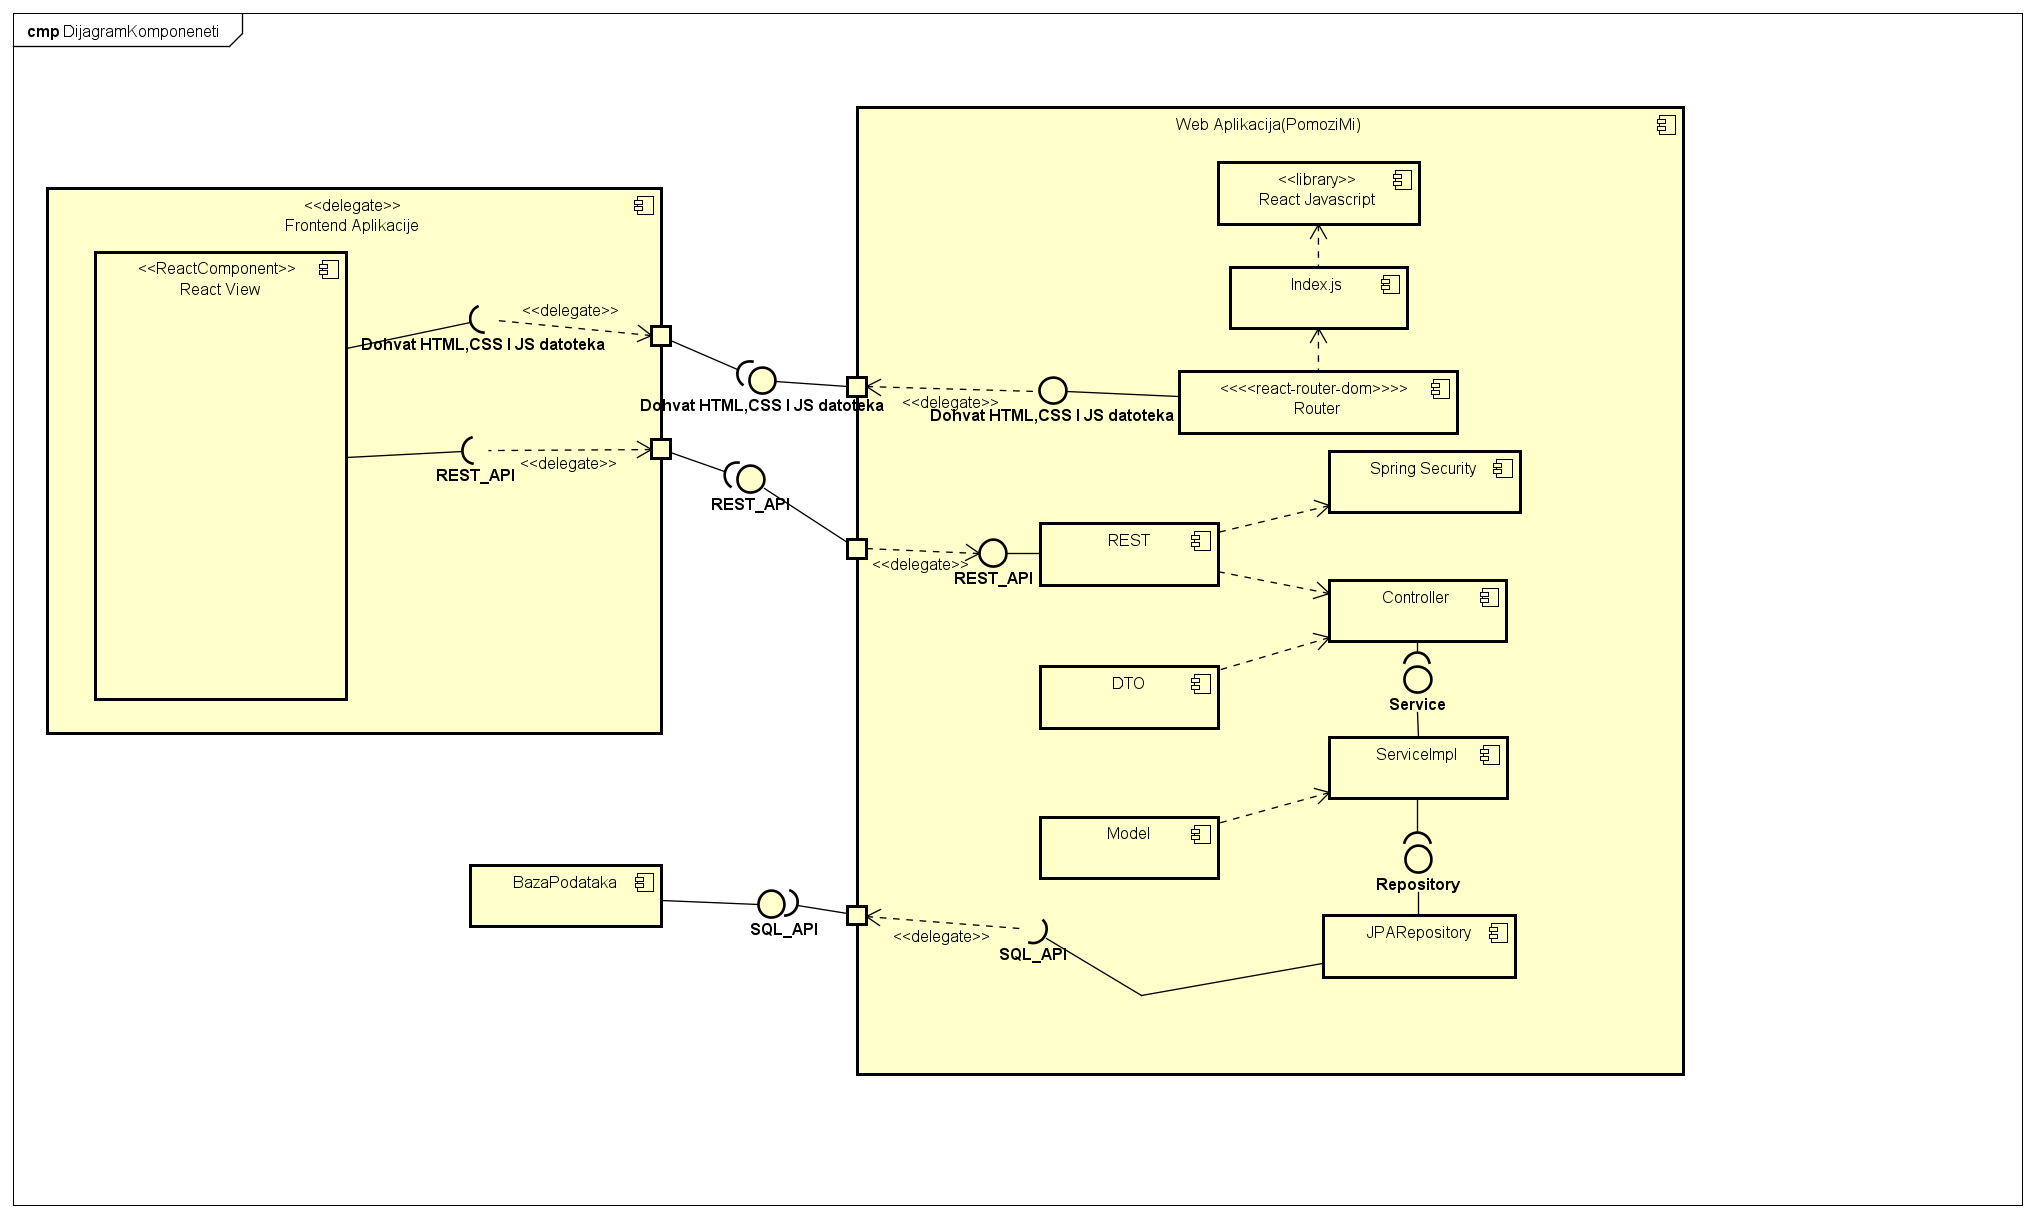
\includegraphics[scale=0.3]{slike/Dijagram Komponeneti.png} %veličina slike u odnosu na originalnu datoteku i pozicija slike
			\centering
			\caption { Dijagram Komponeneti}
			\label{fig:4.12}
			\end{figure}
			
\begin{comment}		
			 \textit{Potrebno je priložiti dijagram komponenti s pripadajućim opisom. Dijagram komponenti treba prikazivati strukturu cijele aplikacije.}
\end{comment}